\chapter{Density Functional Theory (DFT) Methodology for the Calculation of Total Energy}\label{DFT_methods}

\section*{Electronic Structure Calculations}
Modelling electrons requires the use of quantum mechanics, the basis of which is the 
Schr{\"o}dinger equation, which describes the energy of the electrons and nuclei within a material where electrons interact with the positively charged atomic nuclei through an electrostatic potential \cite{Lesar}. The Schr{\"o}dinger equation for a one particle system is given in equation \ref{SE}.
\begin{equation} \label{SE}
\left( - \frac{\hbar}{2m} \nabla^2 + \hat{V} \right)\psi(r,t) = i\text{ } \hbar\frac{\partial \psi}{\partial t}
\end{equation}
However, for systems containing even more than one electron this becomes a very complex problem. This is due to the many electrons in the system interacting with each other as well as with the nuclei. When dealing with such systems, the Born-Oppenheimer approximation is almost universally used. As electrons are fast moving relative to the nuclei, they are considered to be moving in the classical field generated by static nuclei. This decouples the nuclear and electronic degrees of freedom, reducing the problem to solving only the electronic structure of the system. The total energy of the system is then just the sum of the energy of the electrons and the nuclei. The Schr{\"o}dinger equation for a system containing M nuclei and N electrons is shown in equation \ref{many_SE} \cite{Lesar}. This is still a very complex mathematical problem for most systems. For example, $\psi$ in equation \ref{many_SE} for 1 $cm^3$ of a typical metal would be a function of approximately $10^{23}$ variables.
\begin{multline}  \label{many_SE}
\left\{ - \frac{\hbar}{2m} \left( \frac{\nabla_{n_1}^2}{m_1} + ... + \frac{\nabla_{n_M}^2}{m_M}, 
\frac{\nabla_{e_1}^2}{m} + ... + \frac{\nabla_{e_M}^2}{m} \right)
+ V \left( \mathbf{R_1},...,\mathbf{R_M}, \mathbf{r_1}, ..., \mathbf{r_N} \right)
\right\}
\psi (\mathbf{R_1},...,\mathbf{R_M}, \mathbf{r_1}, ..., \mathbf{r_N}, t) \\
= i\hbar \frac{\partial\psi(\mathbf{R_1},...,\mathbf{R_M}, \mathbf{r_1}, ..., \mathbf{r_N},t)}{\partial t}
\end{multline}

\section*{Density Functional Theory (DFT)}\label{DFT_section}
Density functional theory (DFT) is a method to dramatically reduce the computational expense of solving the many-electron Schr{\"o}dinger equation by simplifying the problem. Firstly, DFT considers only the ground state of a system, which dominates most of the properties of a material. This then enables a different formalism of many-body quantum mechanics based on the Hohenberg-Kohn Theorem \cite{hohenberg_kohn}, which states that the ground state energy of a system of electrons in an external potential depends only on the electronic density, $\rho$. 
This results in a dramatic reduction in the complexity of the mathematical problem as the key quantity in the expression is now $\rho$, which is only a function of 3 variables, in comparison to the many-body wavefunction $\psi$ which is a function of 3N variables where N is typically a very large number of electrons within a system. The Kohn-Sham formalism of DFT then produces N non-interacting Schr{\"o}dinger equations, such as that shown in equation \ref{kohn_sham}. 
\begin{equation} \label{kohn_sham}
\left\{ - \frac{\hbar}{2m} \nabla^2 + V[\rho(\mathbf{r})] + V_{xc}[\rho(\mathbf{r})] \right\}\psi(\mathbf{r}) = \epsilon\psi(\mathbf{r})
\end{equation}
\begin{figure}[h!]
  \centering
    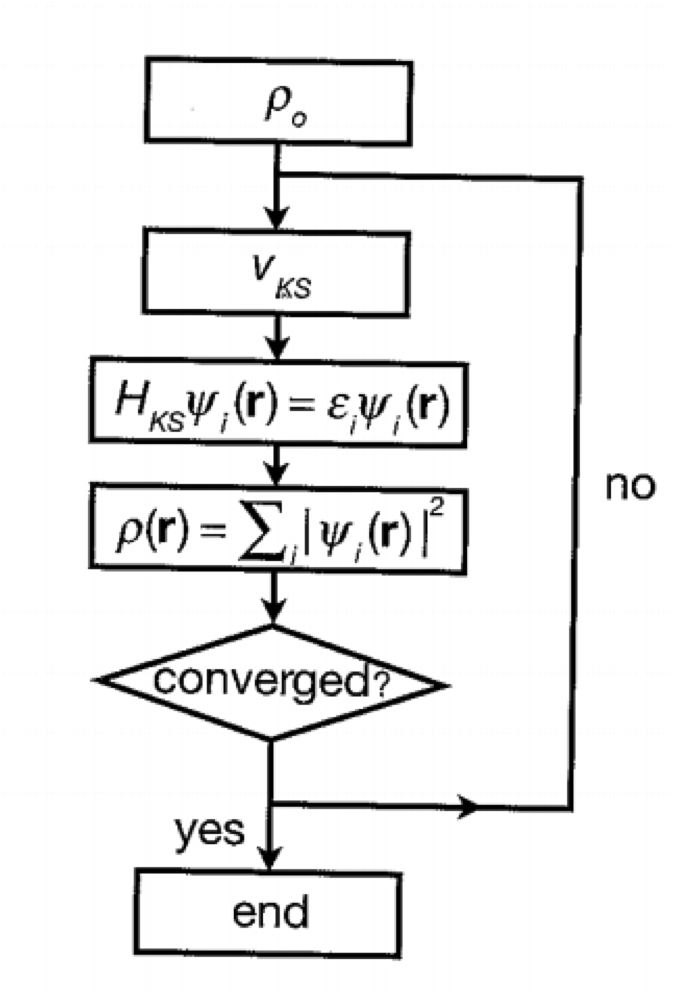
\includegraphics[width=0.3\textwidth]{figures/solving_SE.png}
    \caption{Steps in the solution of the self-consistent field method. Figure taken from reference \citenum{Lesar}.}
  \label{solving_SE}
\end{figure}
The Kohn-Sham method then uses an iterative solution, which is illustrated in figure 
\ref{solving_SE}. An initial guess is made for the set of wavefunctions $\psi_i^0$, an 
initial electron density, $\rho_0$, is then constructed from this where $\rho$ is given by 
equation \ref{rho}. The effective Kohn-Sham potential, $V_{ks}$, is then found based on this value of 
the electron density and equation \ref{kohn_sham2}, where $V_{ext}$ is the external 
potential and $V_{xc} = \frac{\delta E_{xc}}{ \delta \rho(\mathbf{r})}$ where $E_{xc}$ is the 
exchange-correlation function chosen.
\begin{equation}\label{rho}
\rho(\mathbf{r}) = \sum_{i=1}^N |\psi_i(\mathbf{r})|^2
\end{equation}
\begin{equation} \label{kohn_sham2}
V_{ks}(\mathbf{r}) = V_{ext}(\mathbf{r}) + \int \frac{ \rho(\mathbf{r}) } {|\mathbf{r}-\mathbf{r_1}|} d\mathbf{r_1} + V_{xc}(\mathbf{r})
\end{equation}
As $V_{ks}$ is defined by the electron density from the previous step in the iteration cycle, the Hamiltonian includes no direct interaction between electrons. Instead, it describes each electron as moving in an external field based on a fixed electron distribution $\rho(\mathbf{r})$. The Kohn-Sham equation shown in equation \ref{kohn_sham} is then solved with the second and third terms replaced by $V_{ks}$ calculated in equation \ref{kohn_sham2}, to give a new set of wavefunctions and 1-electron orbital energies ($\epsilon$). From this a new $\rho$ is found and then a new $V_{ks}$, until the new value for $\rho$ does not change anymore than a certain prescribed amount after each iteration. This would then be considered to be the ground state energy of the system and this is referred to as a self-consistent process \cite{Lesar}.

\begin{equation}\label{basis_set}
\psi = \sum_j c_j \phi_j
\end{equation}
\begin{equation}\label{plane_wave}
\phi(\textbf{r}) = ce^{i(\textbf{k}+\textbf{G})\cdot \textbf{r}}
\end{equation}
\begin{equation}\label{NAO}
\phi(\textbf{r}) = \frac{u_i(r)}{r} Y_{lm}(\Omega)
\end{equation}

Typically, the wavefunction is expanded as a sum over a set of basis functions as shown in equation \ref{basis_set}.
For solids, the wavefunctions should reflect the periodicity of the system. Plane-waves, such as that shown in equation \ref{plane_wave}, are often chosen for the basis set of a crystal and this is the basis set used in the Vienna Ab-initio Simulation Package (VASP) \cite{VASP}. In the case of the Fritz Haber Institute ab initio molecular simulations (FHI-aims) software package numeric atom-centred orbital (NAO) basis functions, such as that shown in equation \ref{NAO}, are the basis set used. The radial shape, $u_i(r)$, is numerically tabulated and so fully flexible enabling the creation of optimized element-dependent basis sets that are as compact as possible to minimize computational expense. 
To exactly represent the wavefunction may require an infinitely large basis set. In practise, the basis set must be truncated at some point. The consequence of this is that the minimum energy obtained by the iterative method in figure \ref{solving_SE} will always be an upper bound of the true minimum energy of the system. If the size of the basis set is increased, then this minimum value of the energy calculated will decrease further and further towards the true value until convergence is reached such that adding any additional basis states does not change the energy by more than a prescribed amount. 

The FHI-aims package provides pre-constructed default definitions of the basis set for each species depending on the level of accuracy required from the calculations, where these defaults are referred to as `light', `tight' or `really{\textunderscore}tight' settings. Light settings are recommended for initial screening for minimum energy structures or fast pre-relaxations where the relaxed structure can then be used as the input for subsequent more accurate calculations. The developers state that meV-level converged energy differences can be expected for large molecular structures using these settings. Tight settings are stated to guarantee meV-level accuracy for large structures and really{\textunderscore}tight settings are described as only being necessary for individual tests to ensure sufficient accuracy was achieved with less computationally expensive settings \cite{aims}. However when using the VASP software package, the usual practise is to perform convergence tests with calculations with increased energy cut-off for the plane wave basis set.

In periodic DFT calculations, the total energy is also converged with respect to  the number of \textit{k}-points used to sample the Brillouin zone.
Each electron occupies a state of definite $\mathbf{k}$. Therefore, in a periodic crystal structure an infinite number of electrons would result in an infinite number of \textit{k}-points. At each \textit{k}-point, only a finite number of the available energy levels will be occupied. Therefore only a finite number of electrons need to be considered but at an infinite number of \textit{k}-points. In practise, all of these \textit{k}-points are not considered. 
Electron wavefunctions will be almost identical for values of $\mathbf{k}$ that are sufficiently close, so the wavefunctions over a region of reciprocal space can be represented by considering the wavefunction at a single \textit{k}-point. It is therefore sufficient to consider the electronic states at a finite number of \textit{k}-points in order to determine the ground state energy of the solid. This approximation is illustrated in figure \ref{energy_dispersion}. Bloch's Theorem enables the ground state energy to be approximately determined by considering only the number of electrons in the unit cell at a finite number of \textit{k}-points, which are chosen to sample the Brillouin zone appropriately. The choice here is a balance between more \textit{k}-points for a more accurate representation of the Brillouin zone and fewer \textit{k}-points to reduce the computational expense of the calculation \cite{bloch-thesis}. An example of a convergence test for the \textit{k}-grid used in our DFT calculations is shown in Appendix \ref{k-points}. 
\begin{figure}[h!]
  \centering
    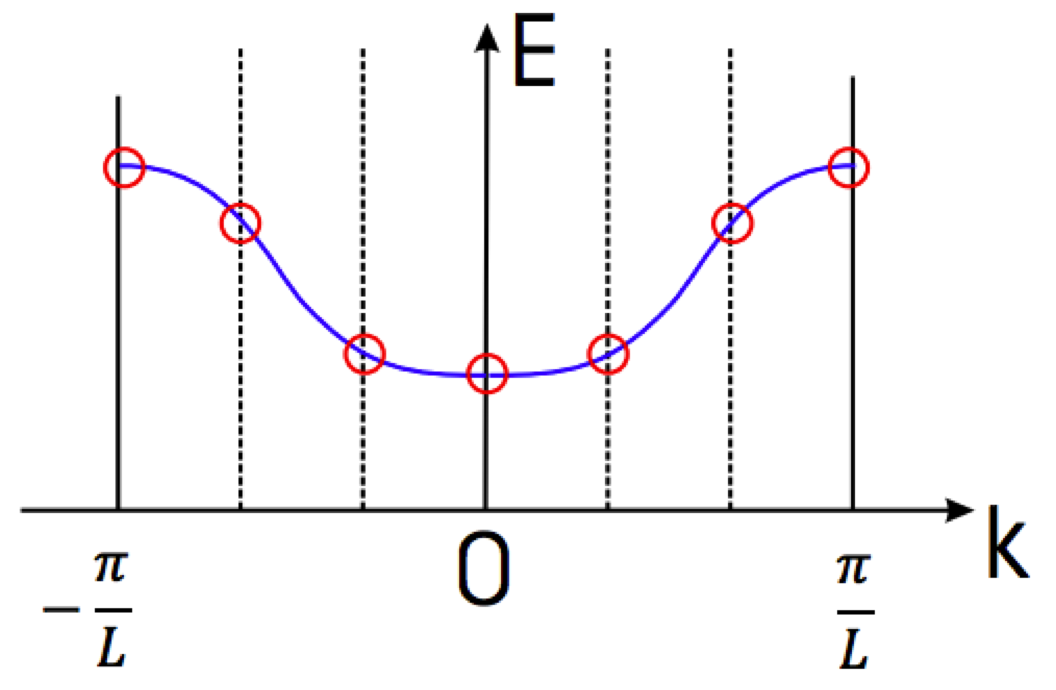
\includegraphics[width=0.4\textwidth]{figures/energy_dispersion.png}
    \caption{The energy dispersion relation for electrons moving in a crystal, illustrating how the function can be approximately represented by a finite number of \textit{k}-points, which form an equally-spaced mesh. Figure adapted from reference \citenum{vasp-slides}.}
  \label{energy_dispersion}
\end{figure}

The fundamental approximation in DFT is the form the unknown exchange-correlation functional, $E_{xc}[\rho]$. The most simple functionals are based on 
the local density approximation (LDA) where an electron with a given local electron density is assumed to 
experience the same many-body response as if the whole material had this same electron density. The next correction to LDA includes the local gradient of the electron density. These methods are referred to as generalised gradient approximations (GGA). These approximations are commonly used for solids and work well for metallic systems which have a fairly uniform electron density. However, they are well know to under-estimate the band gap of semiconductors and insulators. It is possible to ascend the `ladder of DFT Chemical 
accuracy' \cite{ladder} by incorporating more complexity and costly ingredients into the exchange-correlation functional.
Hybrid functionals have been shown to give values for the band gaps of various semiconductors that are in much better agreement with experimental values than those calculated using GGA functionals \cite{hybrid_GGA_CZTS}. In Hybrid approaches there is an interpolation between exact exchange from the Hartree-Fock approximation and DFT exchange-correlation functionals \cite{Lesar}. In this study we made use of the Heyd-Scuseria-Ernzerhof (HSE06) hybrid functional \cite{HSE}.